% --------------------------------------------------------------------------------
\newpage
\section{Contextuality Module}
% --------------------------------------------------------------------------------

% Make general target
\hypertarget{Concepts:ContextualityModule}{}

% Make target for following functions:
\hypertarget{Concepts:IPEMContextualityIndex}{}

\subsection{Introductory description}
% --------------------------------------------------------------------------------

Contextuality measures the pitch commonality between two running
pitch images of the same sound, each having a possible different
echo. In \citeA{article:MusicPerception:Leman:2000}, contextuality
is used to measure the pitch commonality of local (=short echo)
images versus global (=long echo) images. Two types of measurement
are taken into account:
\begin{itemize}
\item
    The first method is based on an \emph{inspection} of the pitch sequence by
    means of a fixed image (or \emph{probe}).
\item
    The second method is based on a \emph{comparison} of the pitch images (each
    having a possible different echo) at running time. This amounts to the
    calculation of the differences, due to the echo, between both running images.
\end{itemize}
Inspection and comparison of echoic pitch images are useful
methods for studying tonal tensions in terms of figure/ground
relationships.\\ In our global chart of image transformation
modules CM is localized in the cognitive section of figure
\ref{Fig:ModulesCM}.

\begin{figure}[h]
    \centering
    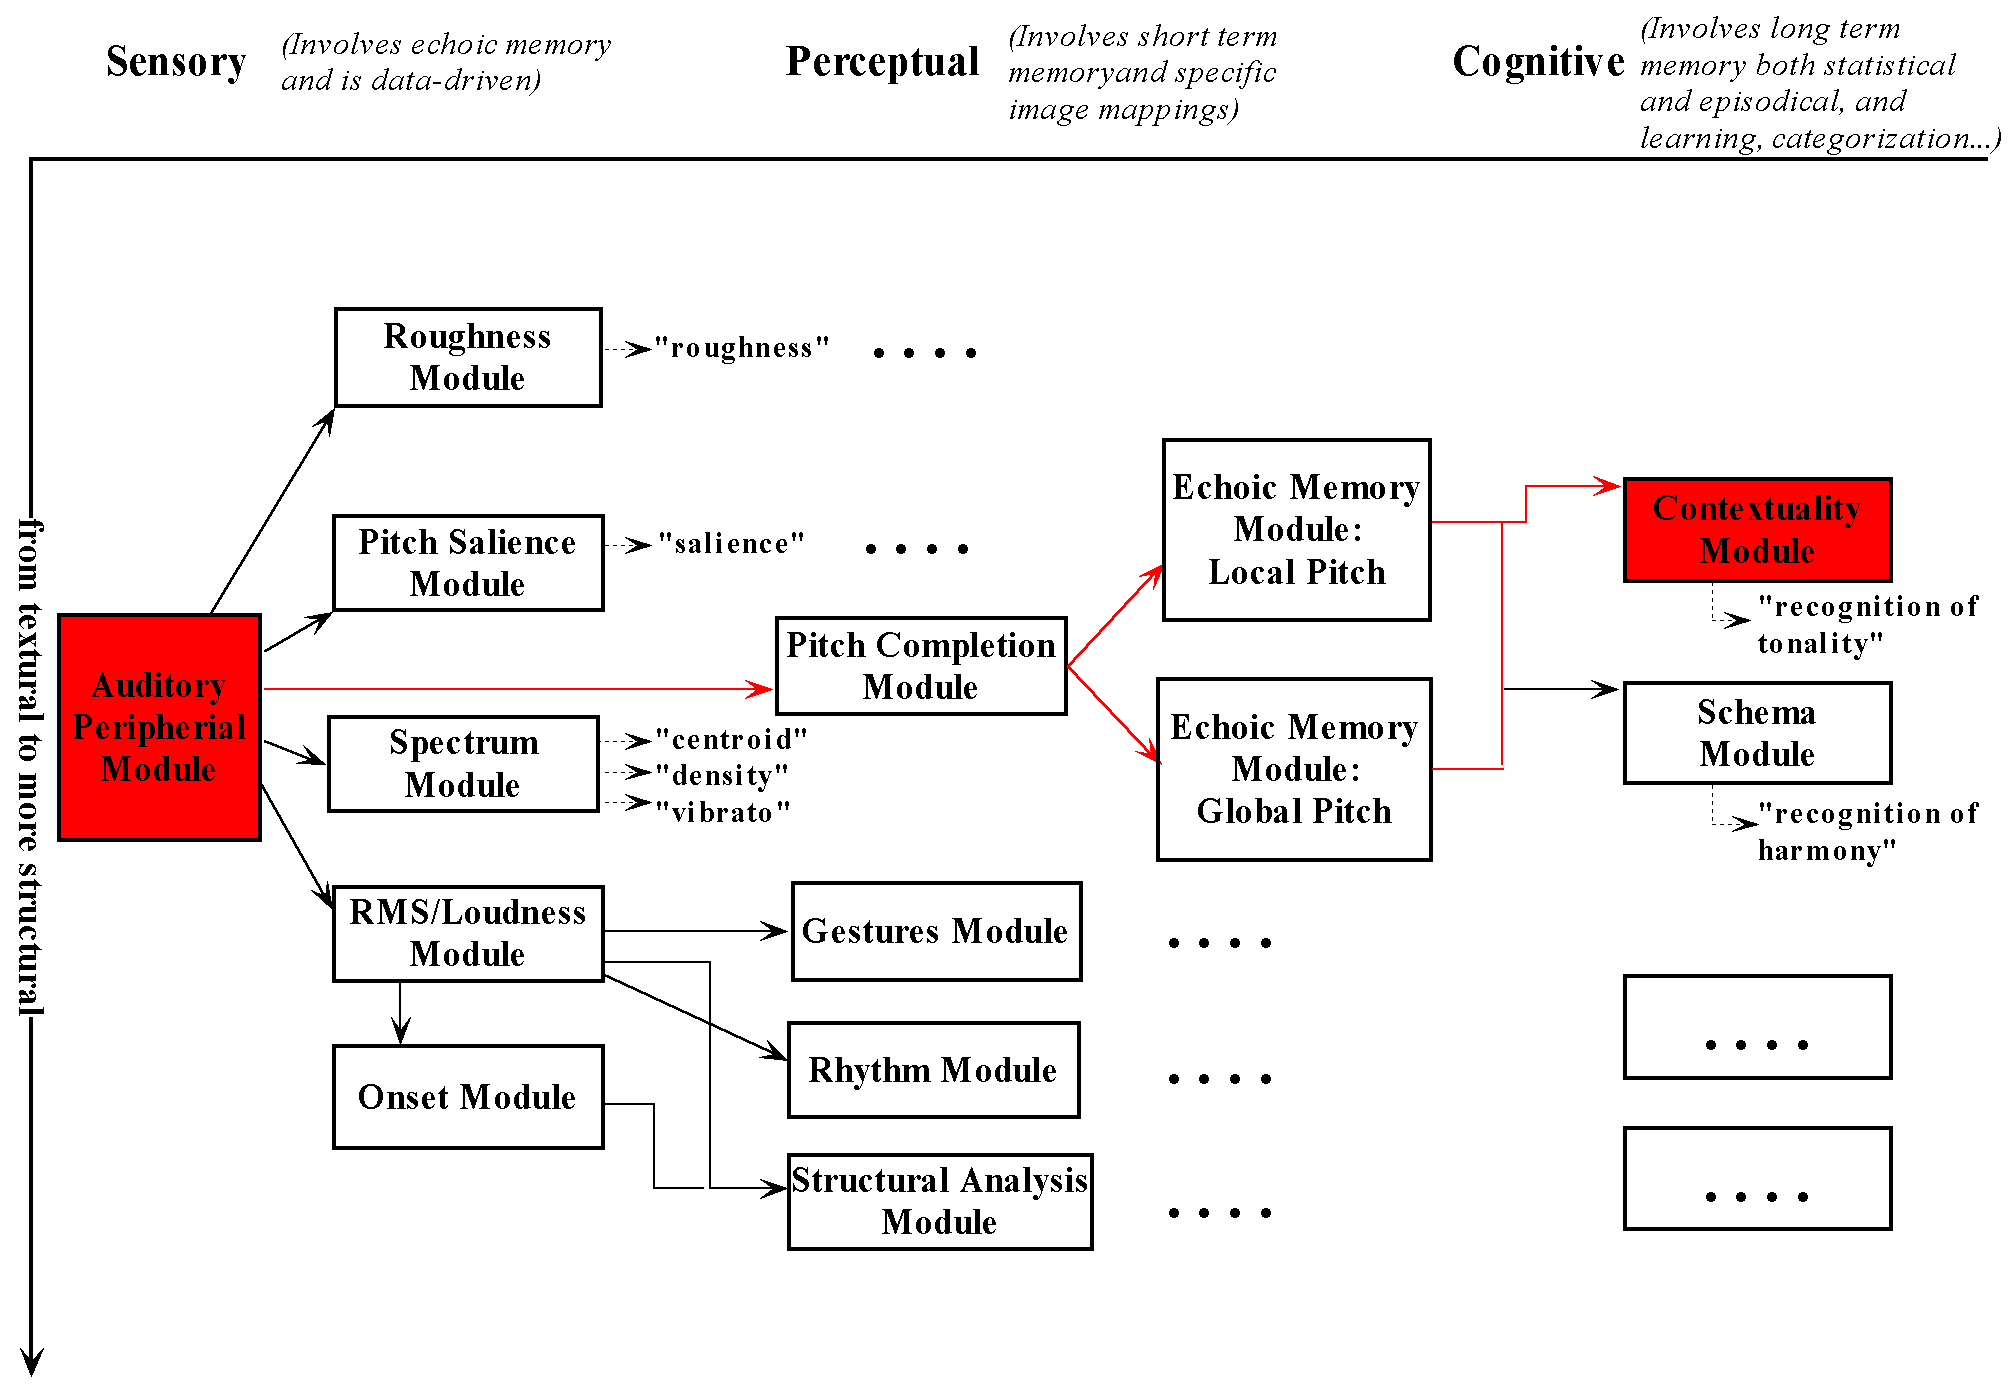
\includegraphics[width=\textwidth]{Graphics/ModulesCM}
    \caption{Chart of image transformation modules, with CM highlighted}
    \label{Fig:ModulesCM}
\end{figure}

Figure \ref{Fig:CMModule} shows the modules involved in the image
transformation and inference process.
\begin{figure}[h]
    \centering
    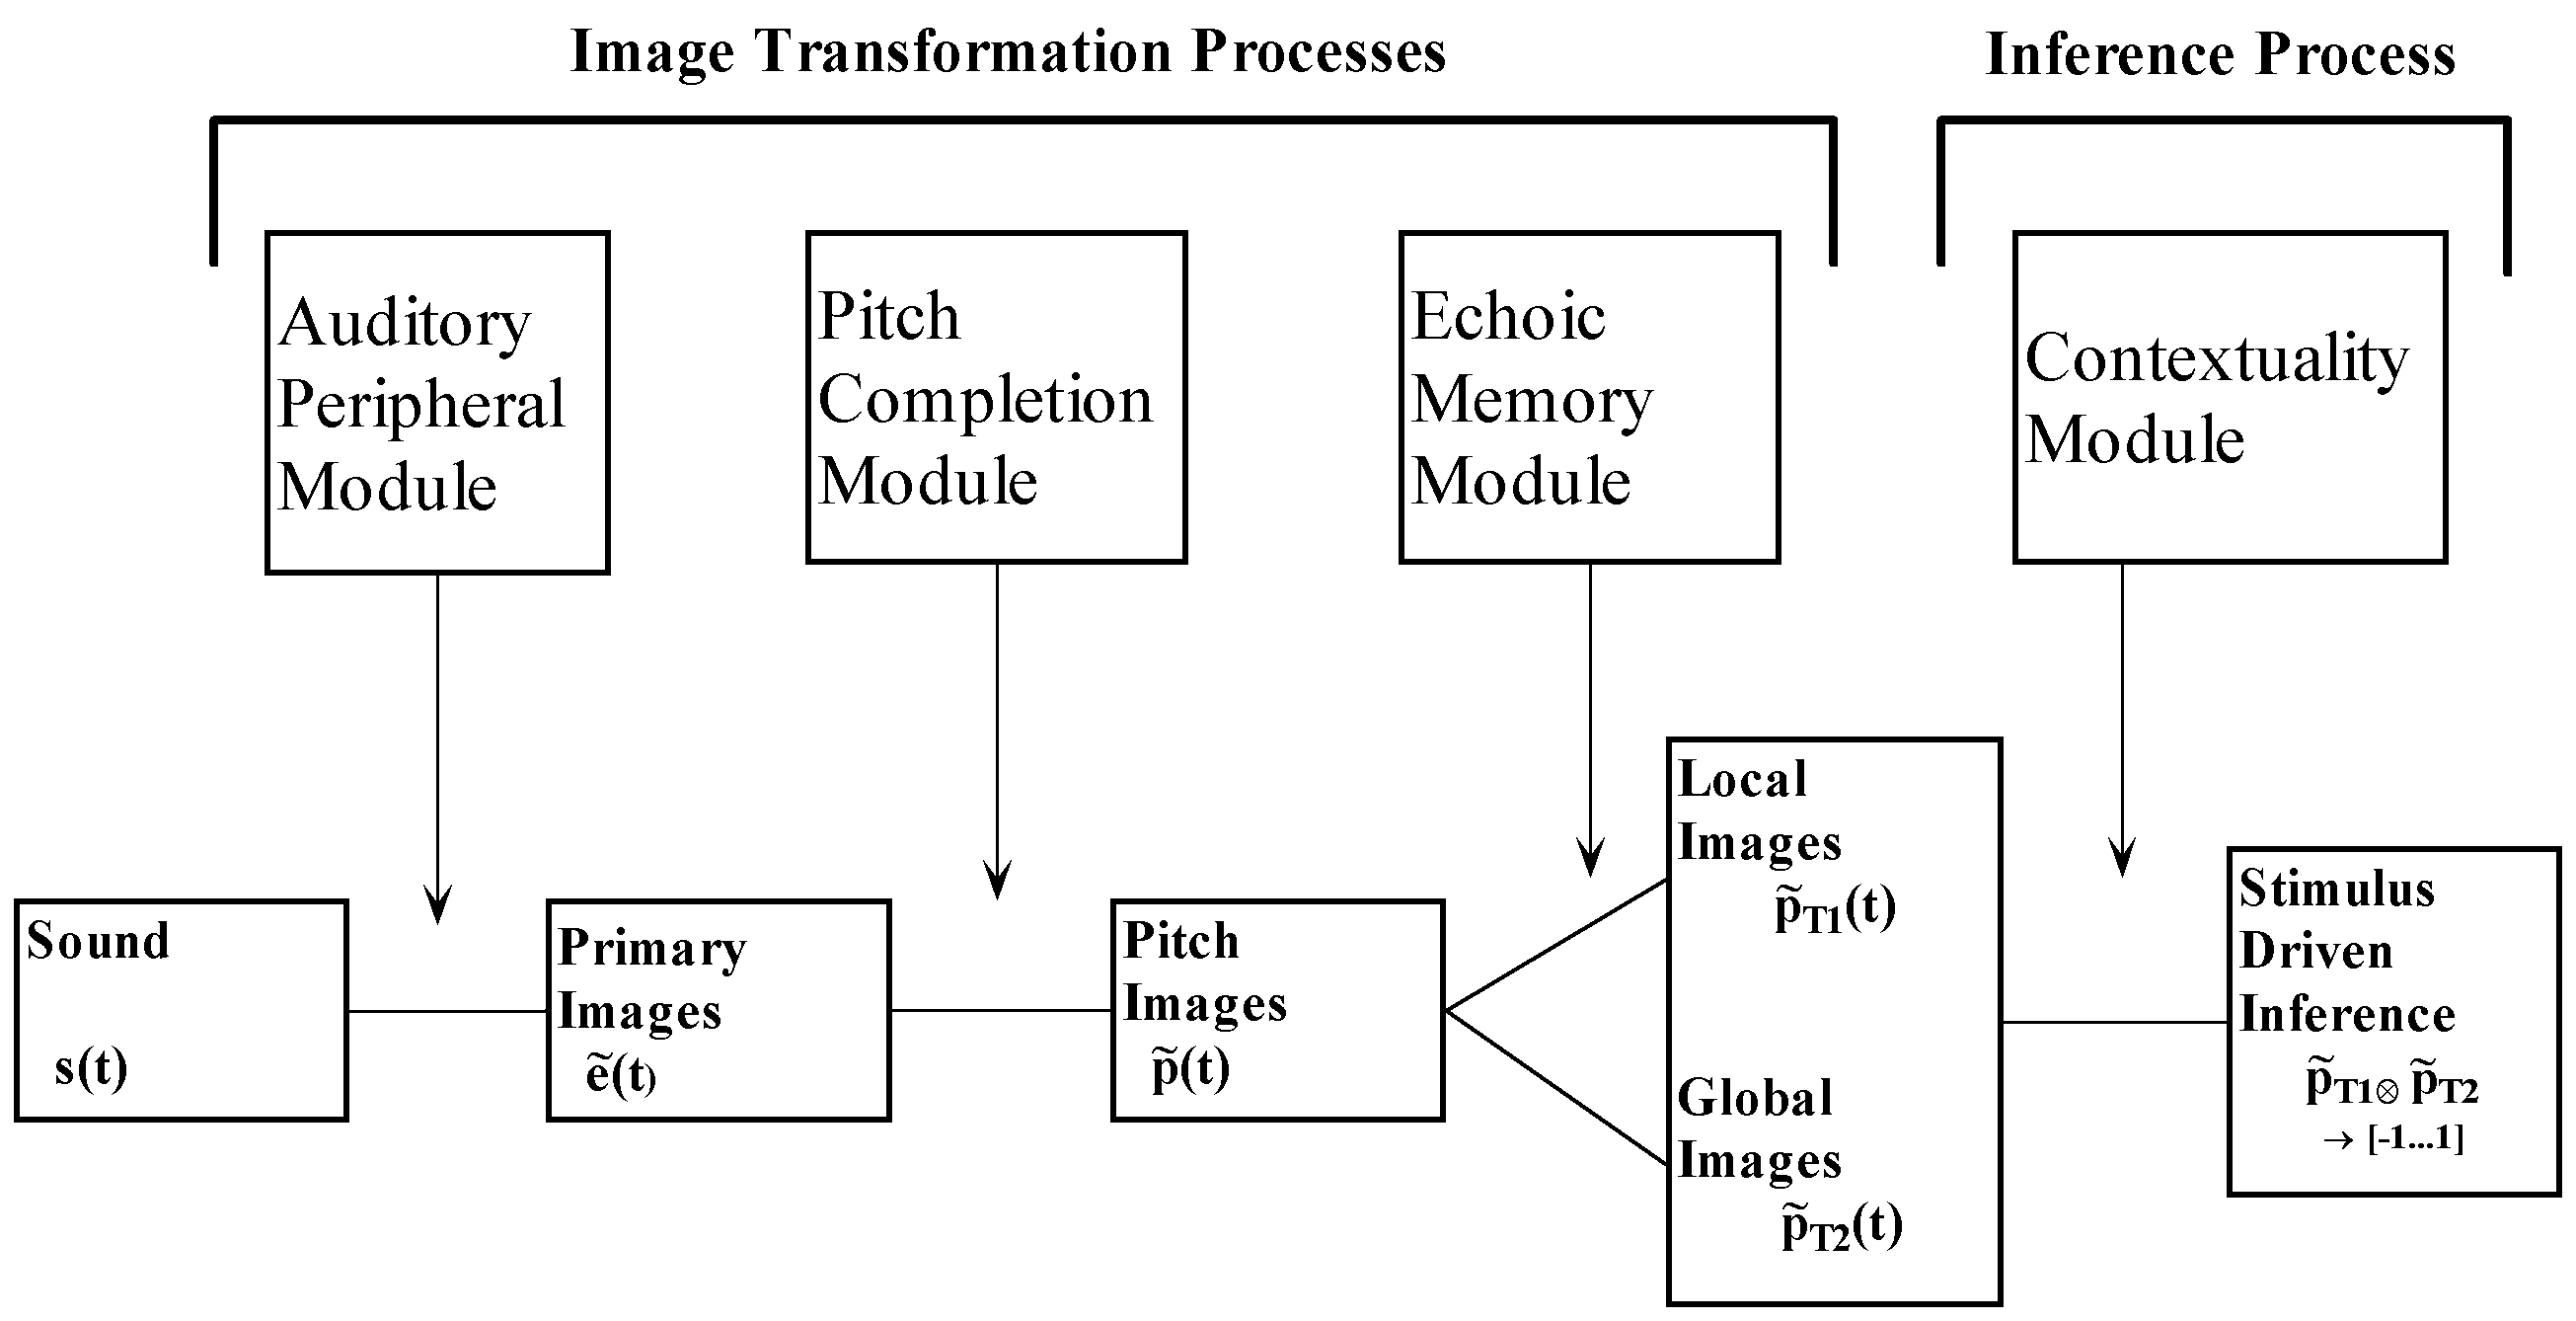
\includegraphics[width=\IPEMDefaultFigureWidth]{Graphics/CMModule}
    \caption{Image Transformation and Inference Process: Contextuality Module}
    \label{Fig:CMModule}
\end{figure}


\subsection{Functional-logical description}
% --------------------------------------------------------------------------------

Contextulatiy realizes a mapping of two images onto a scale:
\begin{equation}
Contextuality: \tilde{p}_{T1} \bigotimes \tilde{p}_{T2} \rightarrow [-1 ... 1]
\end{equation}
where $\tilde{p}$ is a pitch image,
$T1$ and $T2$ are standing for the respective echoes (with T1 $\leq$ T2),
and $\bigotimes$ represents the calculation of a correlation coefficient.
The two methods then correspond to the following mappings:
\begin{itemize}
\item{Inspection:}
    \begin{displaymath}
    Contextuality_{I}: \tilde{p}_{T1}(\tau) \bigotimes \tilde{p}_{T2}(t) \rightarrow [-1 ...
    1]
    \end{displaymath}
    where $\tau$ represents a fixed time instance, typically situated at the end of the
    sound sequence, and $t$ represents the running time.
\item{Comparison:}
    \begin{displaymath}
    Contextulatiy_{II}: \tilde{p}_{T1}(t) \bigotimes \tilde{p}_{T2}(t) \rightarrow [-1 ...
    1]
    \end{displaymath}
    where $t$ represents the running time for both images.
\end{itemize}


\subsection{Signal processing description}
% --------------------------------------------------------------------------------

The Contextuality Module involves several modules.
\begin{itemize}
\item
    The auditory nerve image is calculated using the
    \hyperlink{Concepts:AuditoryPeripheralModule}{Auditory Peripheral
    Module}
\item
    The \hyperlink{Concepts:PitchCompletionModule}{Pitch Completion
    Module} transforms the auditory nerve image into pitch images
\item
    Through the \hyperlink{Concepts:EchoicMemoryModule}{Echoic Memory
    Module} the pitch images undergo the effect of an echo and are
    processed into local and global images
\item
    The Contextuality Module considers two types of contextuality
\end{itemize}


\subsection{Implementation}
% --------------------------------------------------------------------------------

\begin{tabularx}{\linewidth}{llX}
\hyperlink{FuncRef:IPEMContextualityIndex}{IPEMContextualityIndex}
& - & Calculates the contextuality index. Two methods are used:
the method of comparison compares running chords with running tone
center images, while the method of inspection compares a fixed
chord with running chords and running tone center images.
\end{tabularx}


\subsection{Examples}
% --------------------------------------------------------------------------------

Contextuality has been used to simulate the probe-tone experiments
of Krumhansl and Kessler
\cite{article:MusicPerception:Leman:2000,KrumhanslKessler:82}.
%See also \hyperlink{Chapter:ConceptsApplications}{Applications} for more elaborate examples.\\

In what follows, contextuality is applied to the
\IPEMSound{Sounds/SchumannKurioseGeschichte.wav}{short excerpt of
Schumann's Kuriose Geschichte} followed by a 0.1 s period of
silence and an f$\sharp$ Shepard tone. Use the following MATLAB
code to read in the sound file, generate the silence and generate
the Shepard tone f$\sharp$:\\

\begin{IPEMCodeEnvironment}
[s1,fs] = IPEMReadSoundFile('SchumannKurioseGeschichte.wav');
\newline s2 = zeros(1,round(0.1*fs));
\newline NoteFreq = IPEMCalcNoteFrequency('F\#4');
\newline s3 = IPEMShepardTone(NoteFreq,0.5,fs,1,-20);
\end{IPEMCodeEnvironment}\\

Concatenate the 3 sound signals, calculate the auditory nerve
image and from there the periodicity pitch (see also
\hyperlink{Concepts:EchoicMemoryModule}{Echoic Memory Module})
using the following Matlab code:\\

\begin{IPEMCodeEnvironment}
s = [s1 s2 s3];
\newline [ANI,ANIFreq,ANIFilterFreqs] = IPEMCalcANI(s,fs);
\newline [PP,PPFreq,PPPeriods,PPFANI] = IPEMPeriodicityPitch(ANI,ANIFreq,[],[],[],1);
\end{IPEMCodeEnvironment}\\

Then finally, the function
\hyperlink{FuncRef:IPEMContextualityIndex}{IPEMContextualityIndex}
 is applied for the context analysis.\\

\begin{IPEMCodeEnvironment}
[Chords,ToneCenters,LocalInspection,GlobalInspection,LocalGlobalComparison] = ...
\newline IPEMContextualityIndex(PP,PPFreq,PPPeriods,[],0.1,1.5,[],1);
\end{IPEMCodeEnvironment}\\

In this example, \IPEMCodeExtract{PP} contains the periodicity
pitch image of the concatenated sounds, \IPEMCodeExtract{PPFreq}
contains the sampling rate, \IPEMCodeExtract{PPPeriods} contains
the analyzed periods, and the fourth argument specifies the
location of the fixed image. Here, it is left blank, which
defaults to the end of the signal. The local and global echoes are
set to 0.1 s and 1.5 s, respectively, and the plot flag is set to
1.\\

Figure \ref{Fig:ContextualityPitchImages} shows the periodicity
pitch image of the Schumann excerpt followed by the Shepard tone,
the local pitch image, and the global pitch image.\\
The method based on inspection has been applied to the local and
the global pitch images.\\

\IPEMCodeExtract{LocalInspection}
(fig. \ref{Fig:ContextualityLocalInspection}) contains the results
of inspecting the local images with the fixed (local) image. The
graph shows the similarity of the Shepard probe tone of
f$\sharp$ within the Schumann excerpt at a local level.\\

\IPEMCodeExtract{GlobalInspection}
(fig. \ref{Fig:ContextualityGlobalInspection}) contains the
results of inspecting the global images with the fixed (local)
image. The graph shows the similarity of the Shepard probe tone of
f$\sharp$ within the Schumann excerpt at a more global pitch
level.\\

\IPEMCodeExtract{LocalGlobalComparision}
(fig. \ref{Fig:ContextualityLocalGlobalComparison}) contains the
results of comparing the local images with the global images over
the whole piece. It shows the degree in which the local pitch
images (= the level of individual tones and chords) fit with the
global pitch images (= the level of the tone context). At points
where the local image deviates from the global image, such as in a
tonal movement, there will be a low correlation. Inversely, at
points where the local image confirms the global image, there will
be a high correlation.\\

\begin{figure}[h]
    \centering
    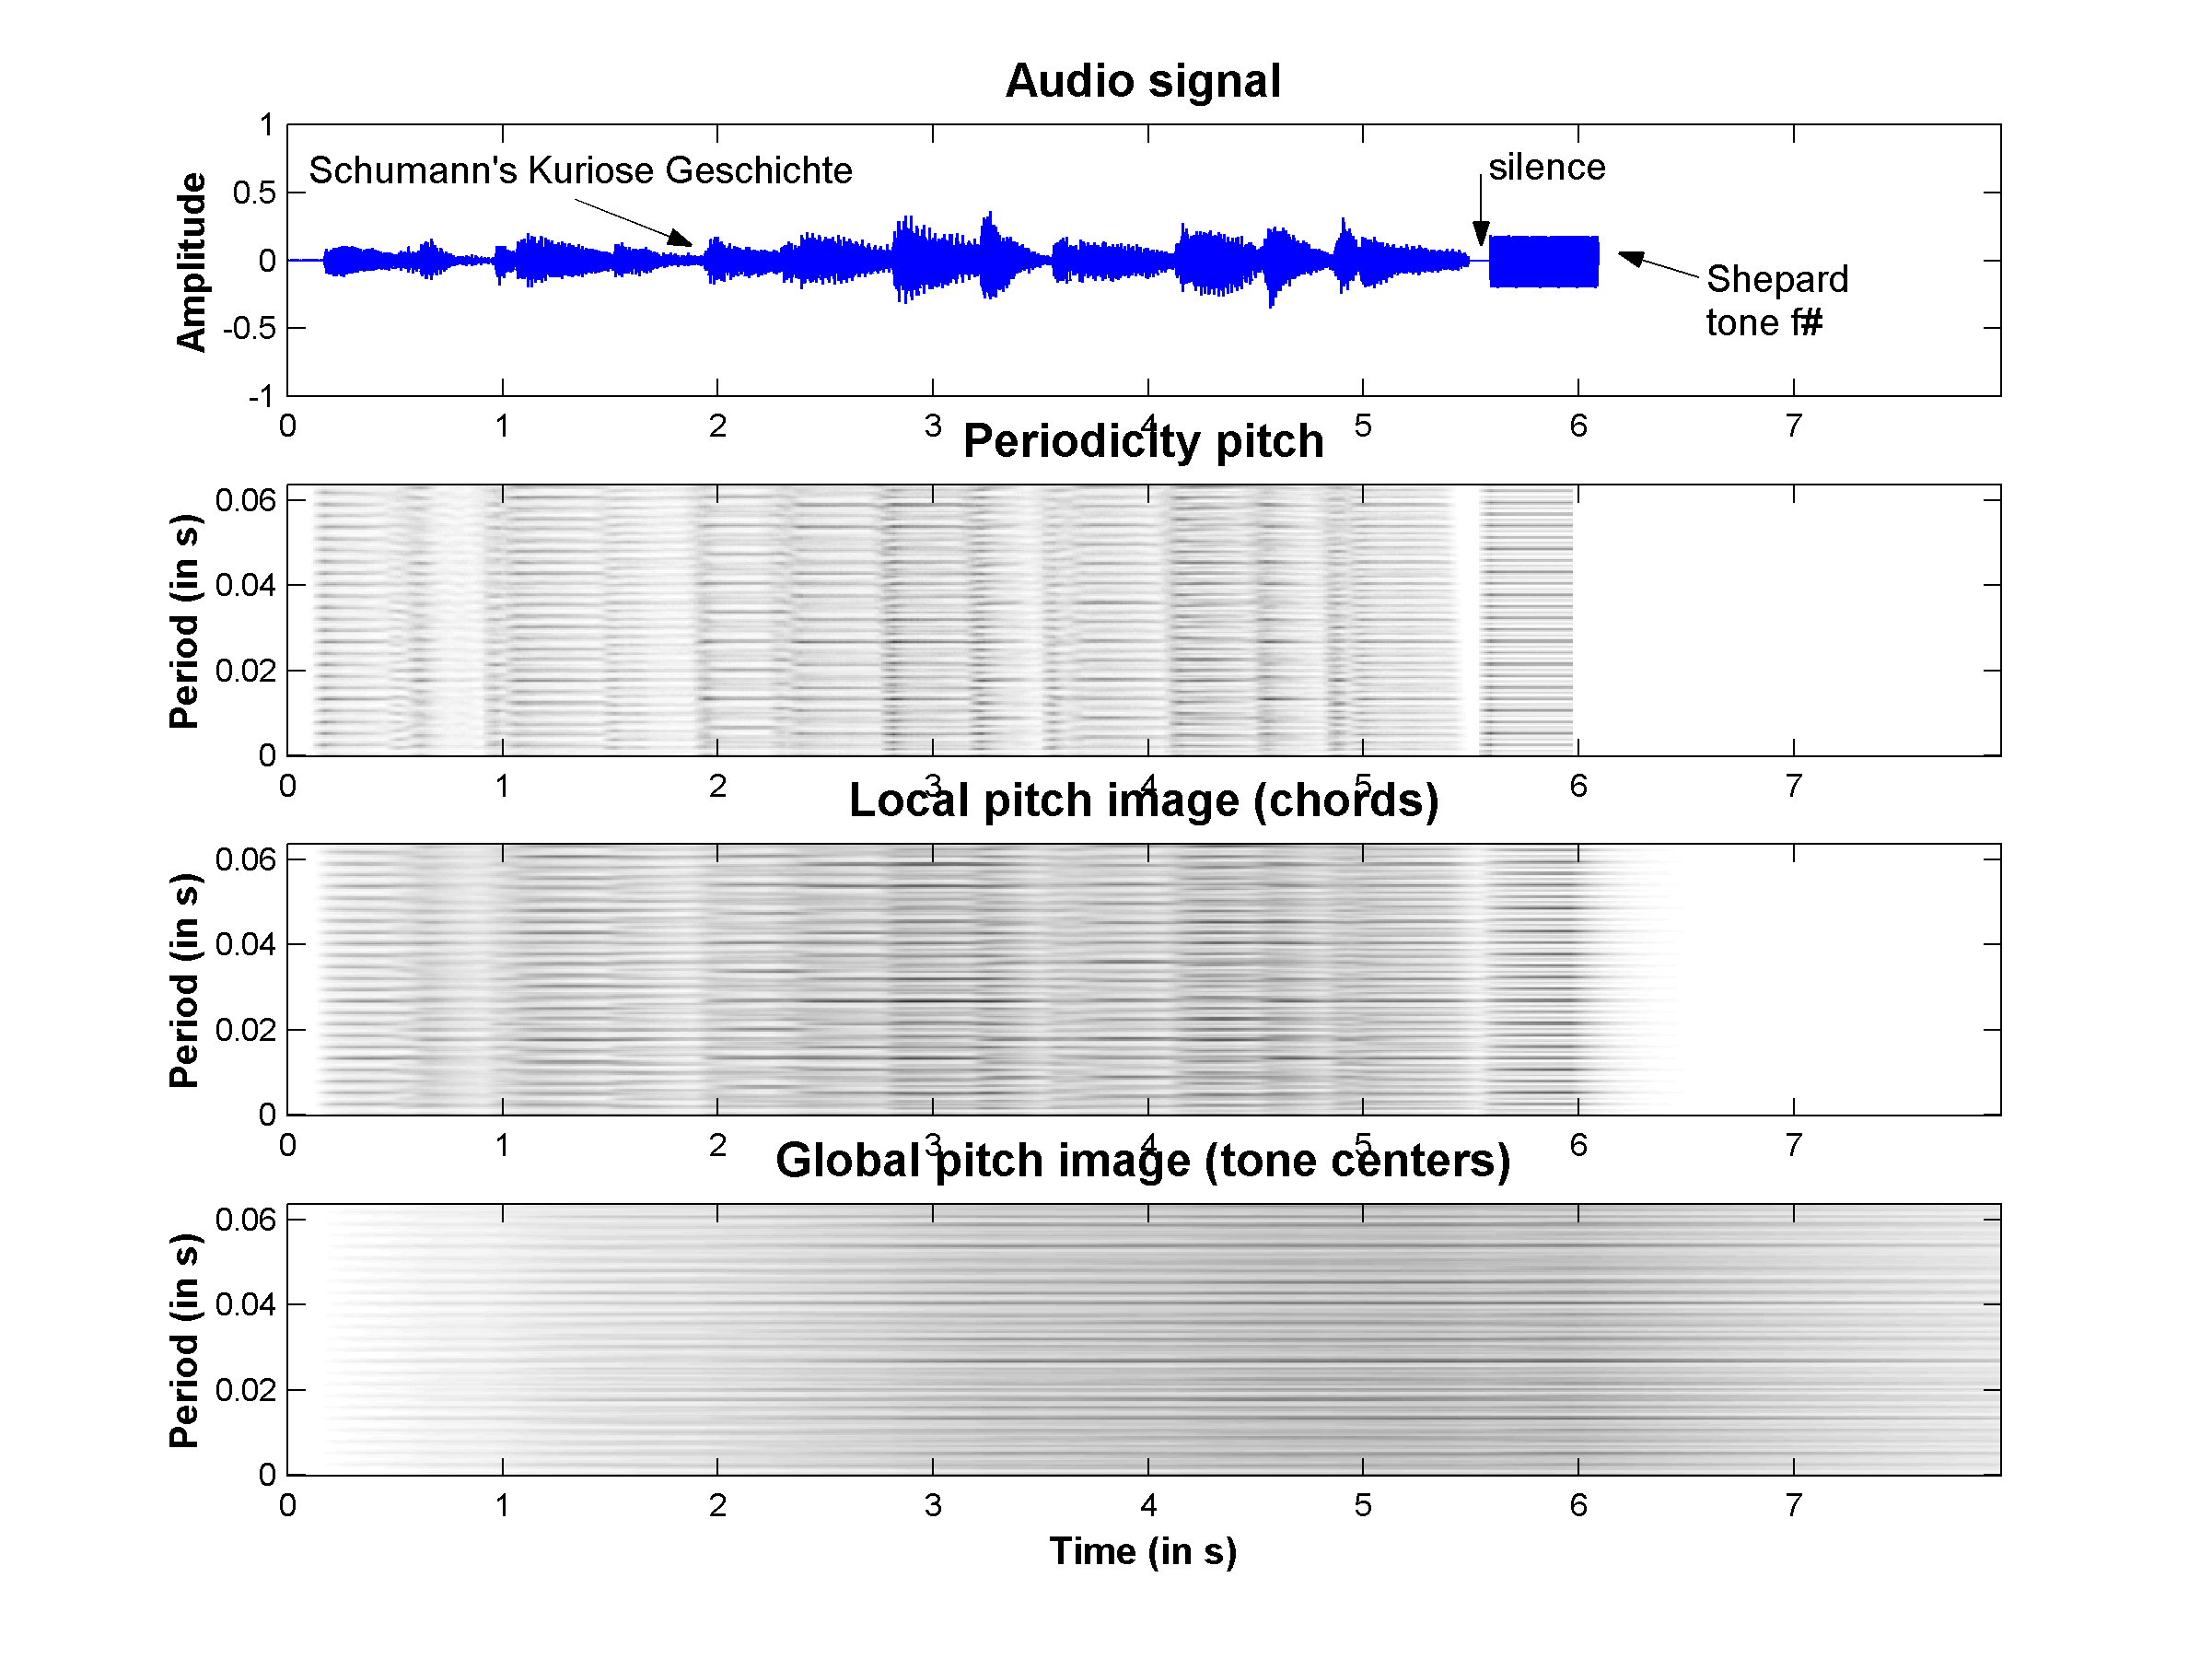
\includegraphics[width=\IPEMDefaultFigureWidth]{Graphics/ContextualityPitchImages}
    \caption{Pitch images for the excerpt of Schumann's Kuriose
    Geschichte followed by a small period of silence and a Shepard
    probe-tone of f$\sharp$. From top to bottom: the analyzed
    audio signal, the periodicity pitch image, the local pitch image and
    the global pitch image.} \label{Fig:ContextualityPitchImages}
\end{figure}

\begin{figure}[h]
    \centering
    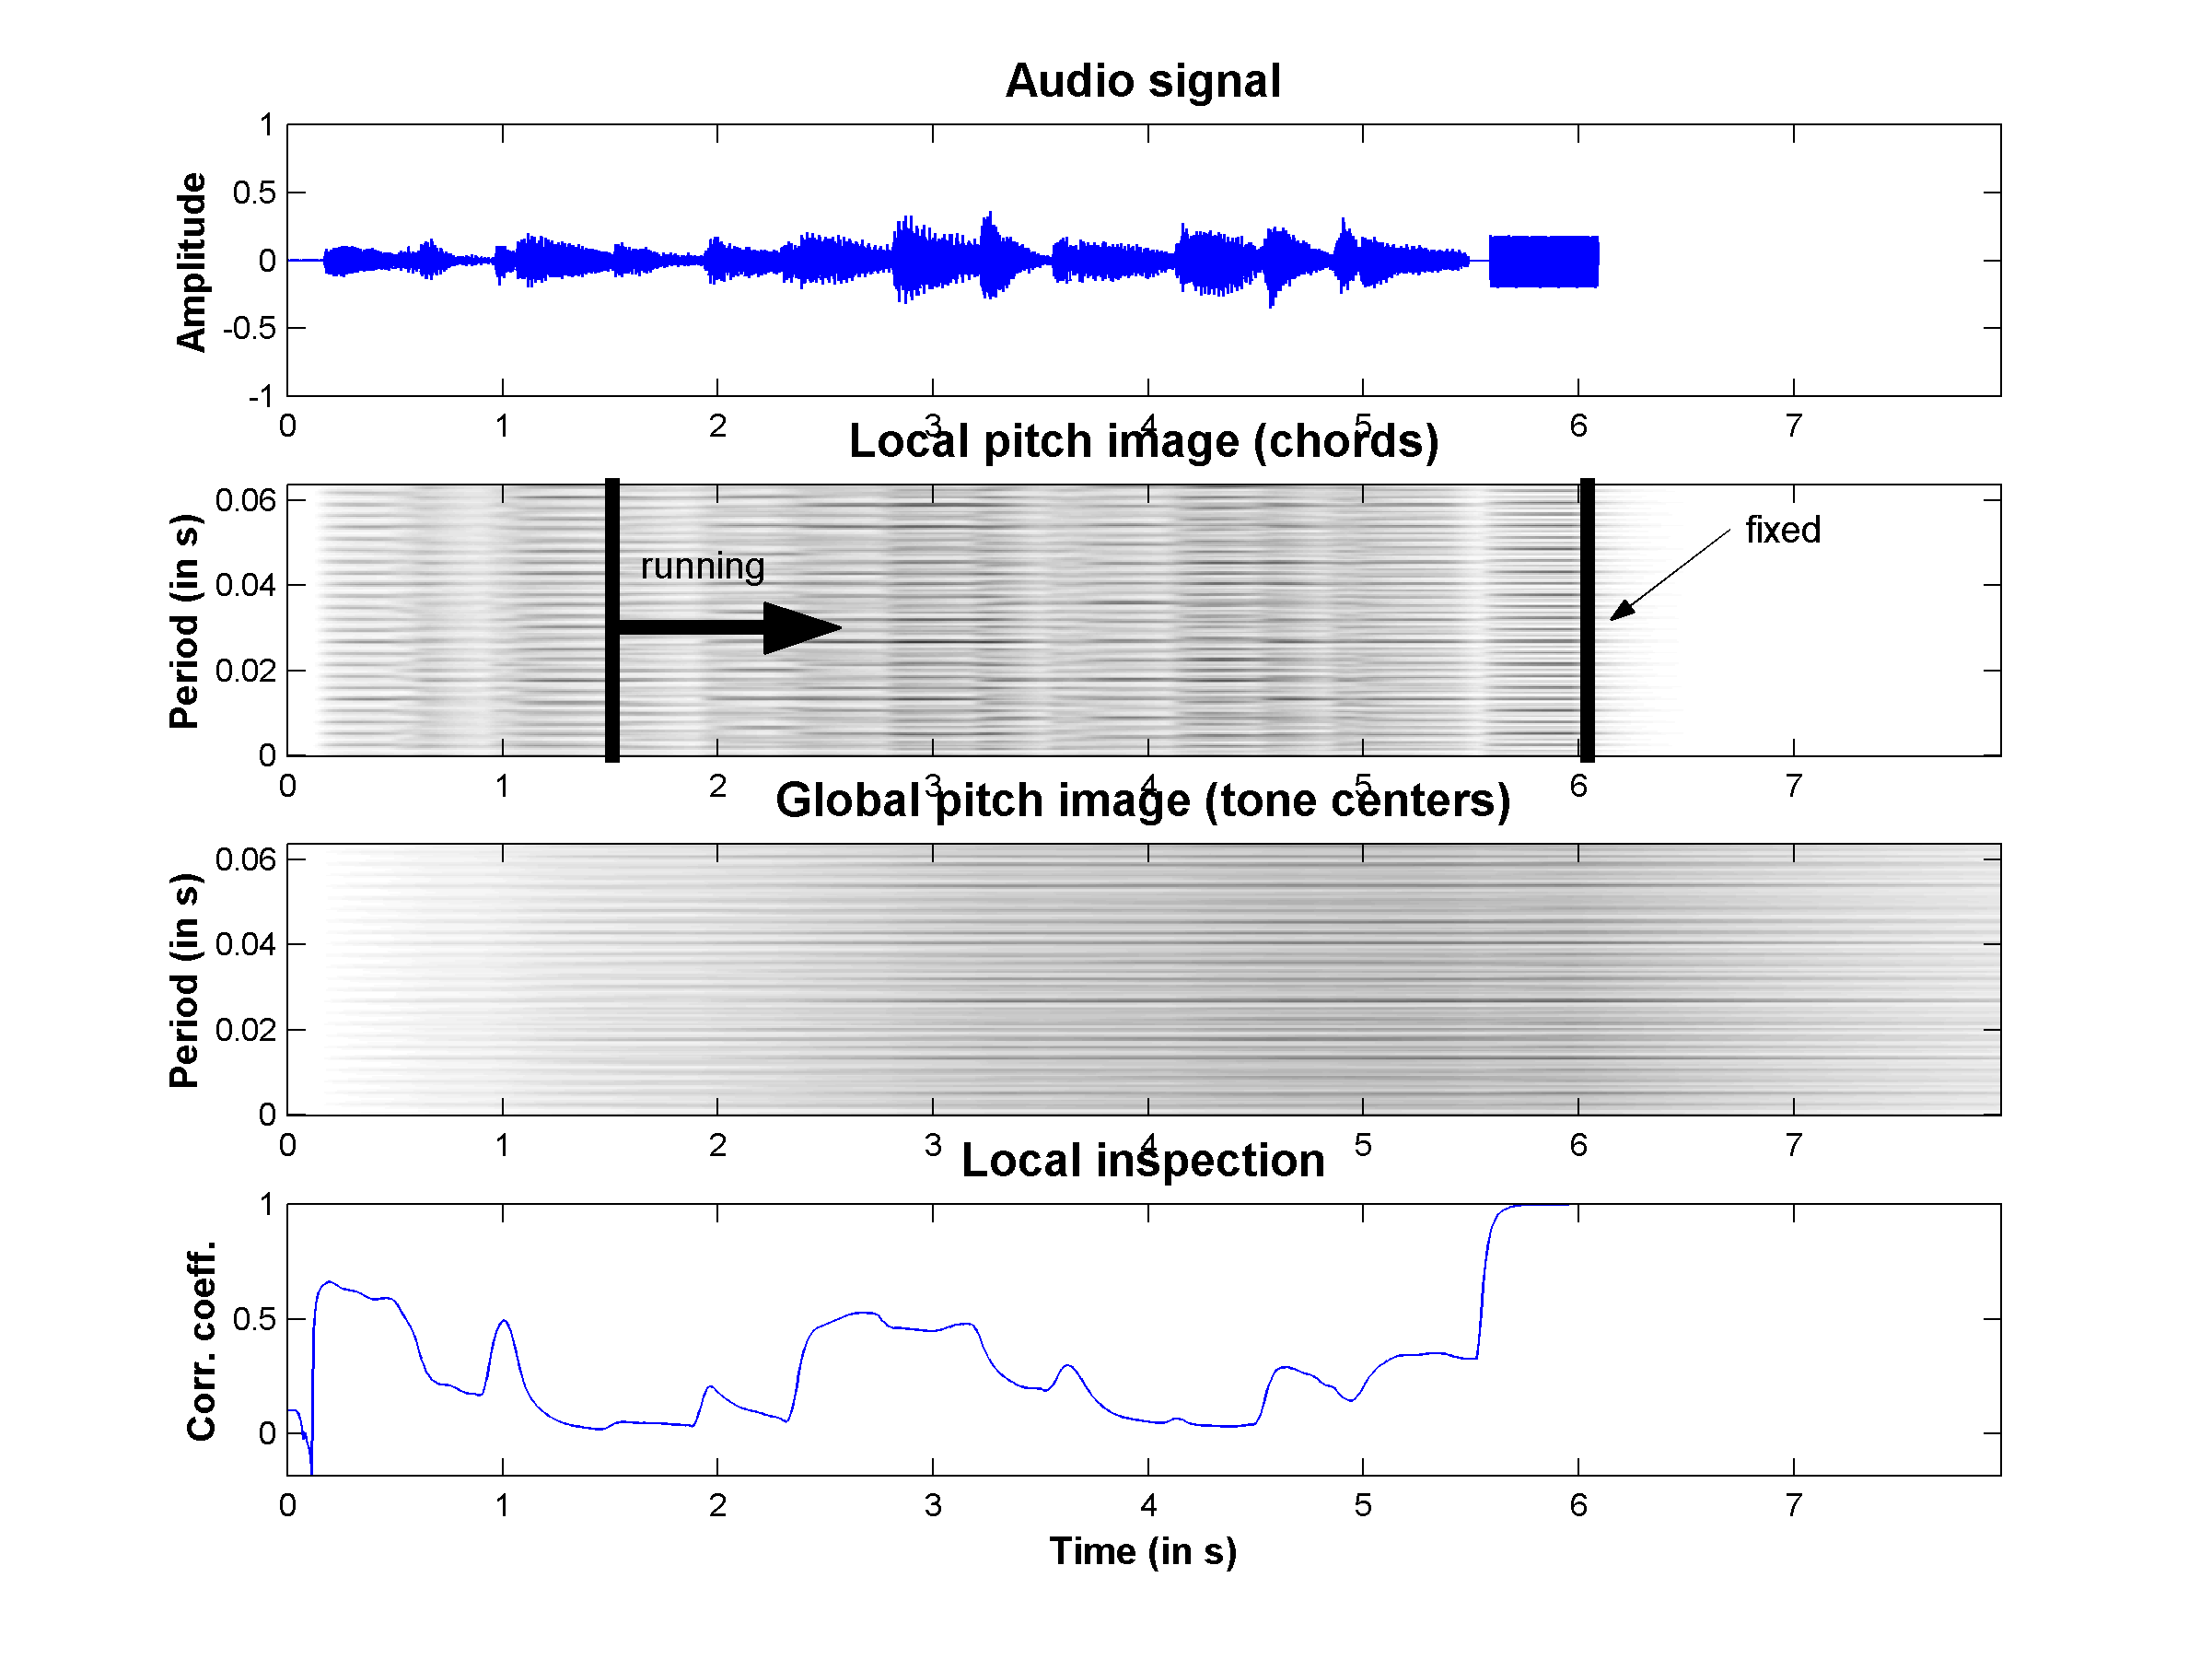
\includegraphics[width=\IPEMDefaultFigureWidth]{Graphics/ContextualityLocalInspection}
    \caption{Inspection of Schumann's Kuriose Geschichte followed
    by a small period of silence and a Shepard probe-tone of
    f$\sharp$. Inspection of local images. From top to bottom:
    audio signal, local pitch image, global pitch image and local
    inspection.} \label{Fig:ContextualityLocalInspection}
\end{figure}

\begin{figure}[h]
    \centering
    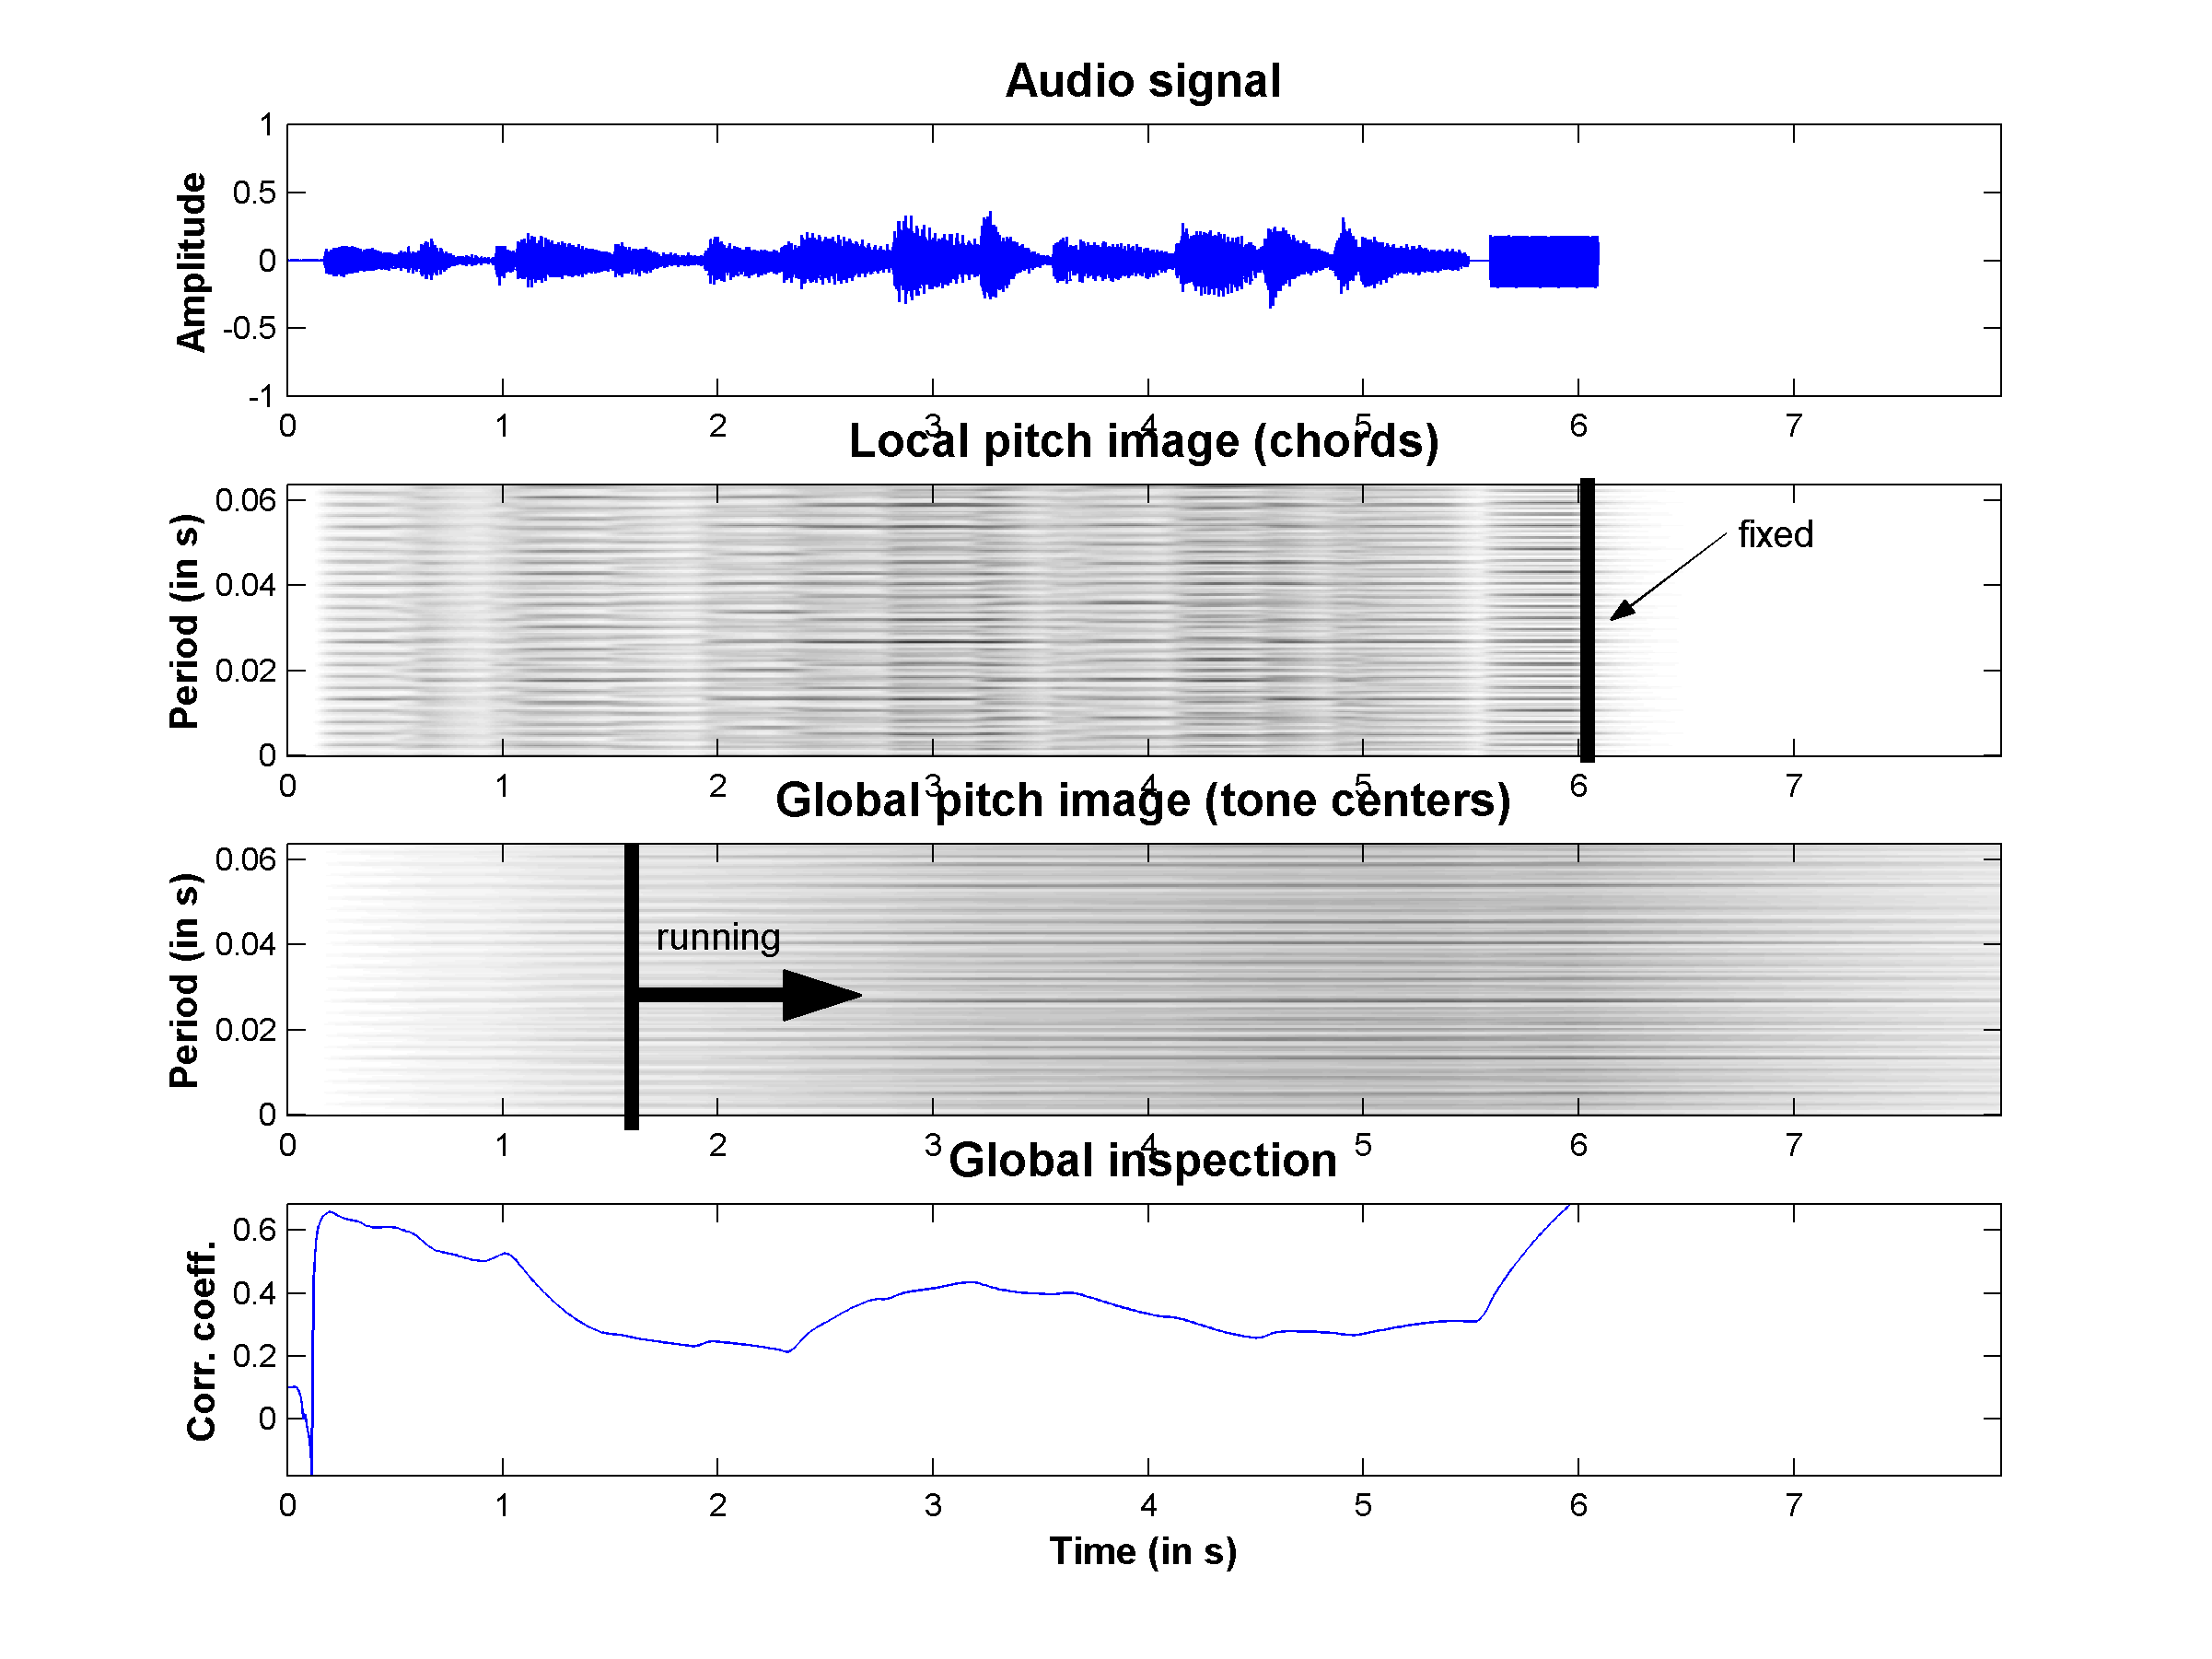
\includegraphics[width=\IPEMDefaultFigureWidth]{Graphics/ContextualityGlobalInspection}
    \caption{Inspection of Schumann's Kuriose Geschichte followed
    by a small period of silence and a Shepard probe-tone of
    f$\sharp$. Inspection of global images. From top to bottom:
    audio signal, local pitch image, global pitch image and global
    inspection} \label{Fig:ContextualityGlobalInspection}
\end{figure}

\begin{figure}[h]
    \centering
    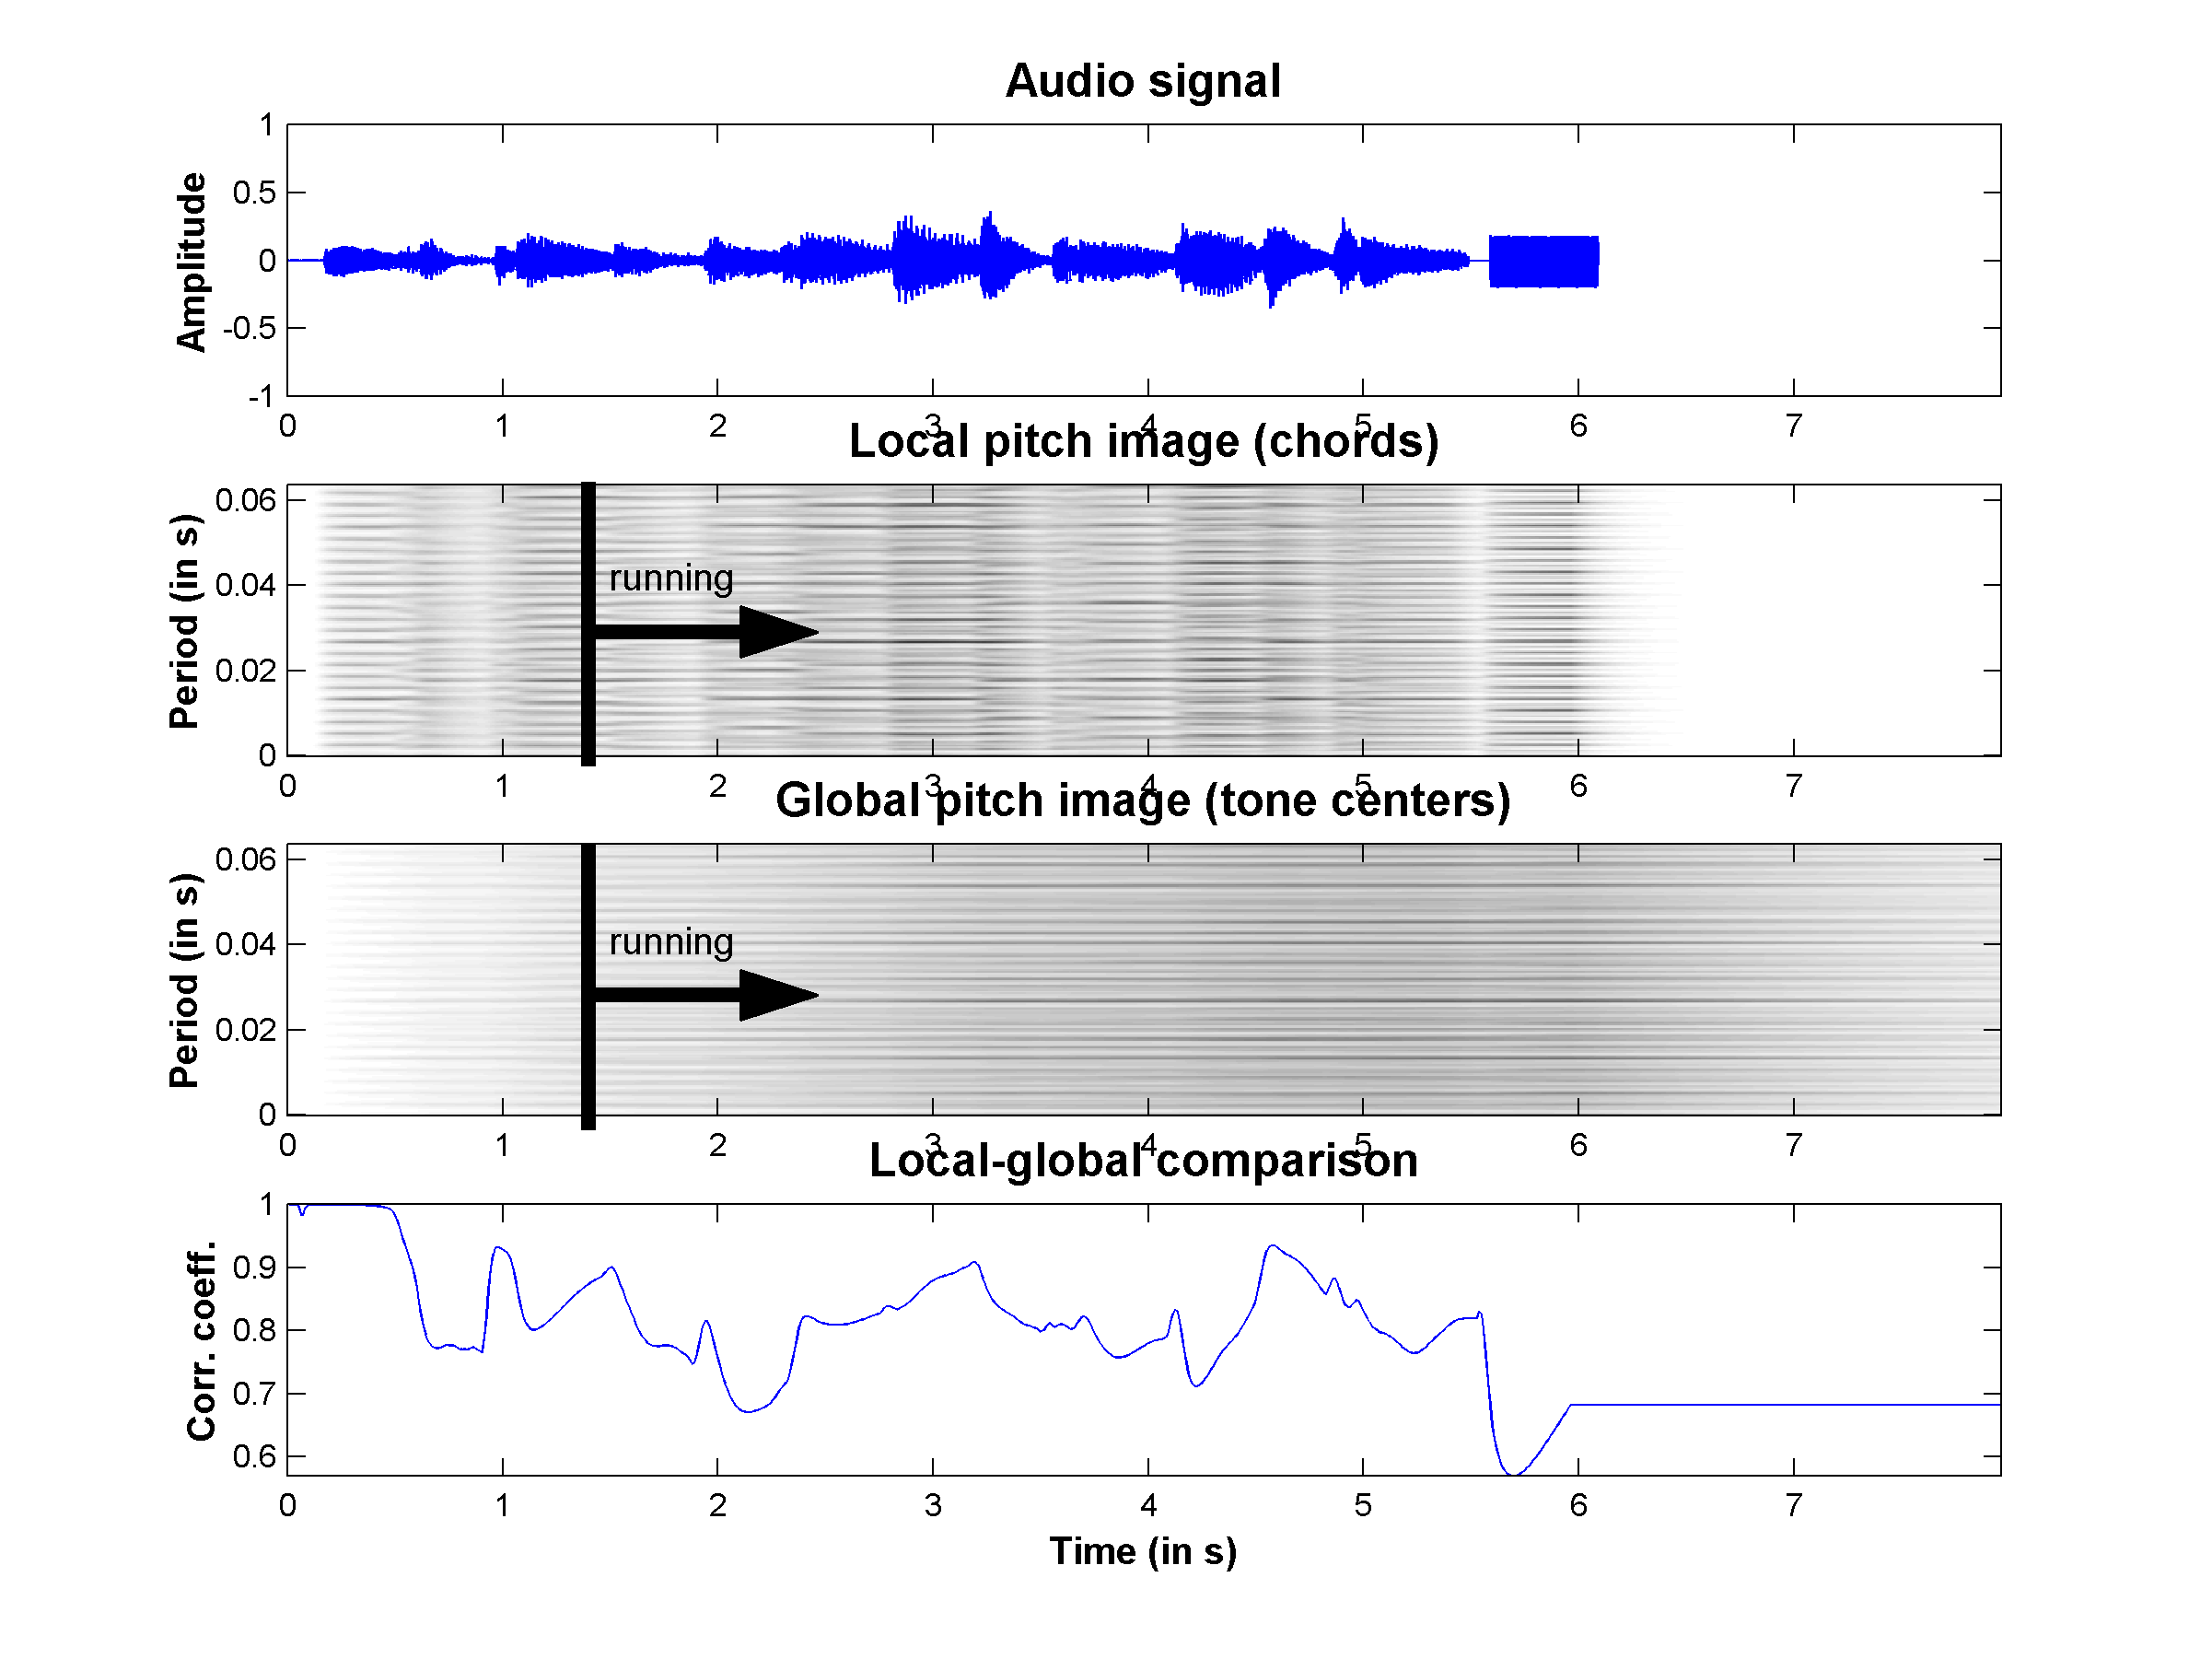
\includegraphics[width=\IPEMDefaultFigureWidth]{Graphics/ContextualityLocalGlobalComparison}
    \caption{Comparison of the local and global pitch images of
    Schumann's Kuriose Geschichte followed by a small period of
    silence and a Shepard probe-tone of f$\sharp$. From top to
    bottom: audio signal, local pitch image, global pitch image
    and comparison between local and global pitch images.}
    \label{Fig:ContextualityLocalGlobalComparison}
\end{figure}
